\documentclass[tikz,border=5pt]{standalone}
\usepackage{amsmath}
\begin{document}
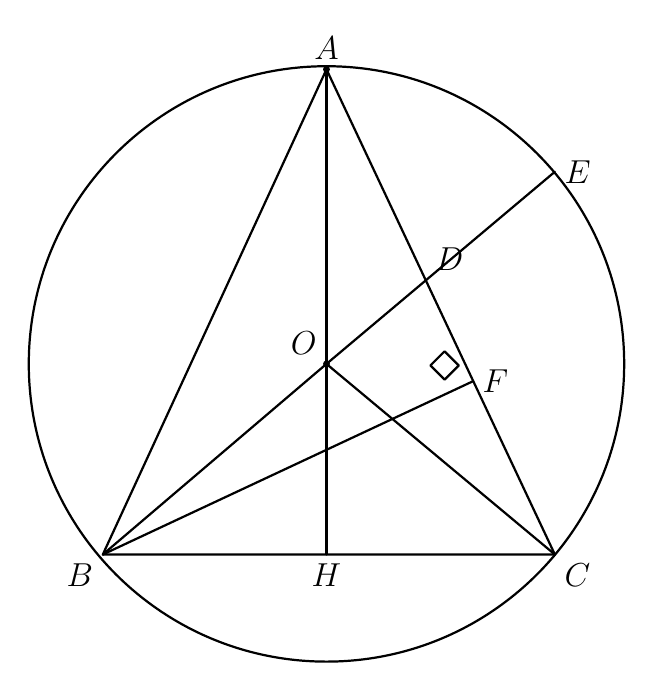
\begin{tikzpicture}[x=0.02cm,y=-0.02cm,line cap=round,line join=round,font=\large]

% 坐标（像素近似，y 轴向下）
\coordinate (A) at (217,67);
\coordinate (B) at (75,375);
\coordinate (C) at (362,375);
\coordinate (H) at (217,375);
\coordinate (O) at (217,254);
\coordinate (D) at (280,201);
\coordinate (E) at (362,132);
\coordinate (F) at (310,265);

% 外接圆
\draw[line width=0.8pt] (217,254) circle (189);

% 三角形 ABC
\draw[line width=0.8pt] (A) -- (B) -- (C) -- cycle;

% 高 AH：AO 已改为实线，OH 保持实线
\draw[line width=0.8pt] (A) -- (O);
\draw[line width=0.8pt] (O) -- (H);

% 其余线段
\draw[line width=0.8pt] (B) -- (O) -- (C);
\draw[line width=0.8pt] (O) -- (E);
\draw[line width=0.8pt] (B) -- (F);

% 直角标记
\draw[line width=0.8pt] (283,255) -- (292,246) -- (301,255) -- (292,264) -- cycle;

% 点（原图中 A、O 等处的小圆点）
\fill (A) circle (2.2);
\fill (O) circle (2.2);

% 标签
\node[above] at (A) {$A$};
\node[below left] at (B) {$B$};
\node[below right] at (C) {$C$};
\node[below] at (H) {$H$};
\node[above left] at (O) {$O$};
\node[above right] at (D) {$D$};
\node[right] at (E) {$E$};
\node[right] at (F) {$F$};

\end{tikzpicture}
\end{document}
